\chapter{Verification and validation}
\label{ch:verification}

\section{Overview}

In order to test the effectiveness of the additions to the original algorithm, games must be run with different parameters (e.g. with and without the neural network ghost controller, wit more or less training cycles, etc).  Since the variation of the results for a given parameters set is high, many games must be run for each and an average obtained.  This results in easily hundreds of games that need to be played to evaluate the project.  The games must be played in real time, as the Pac-Man controller takes the full 40~ms available to it each time step.  The maximal length of a game is limited to 16 minutes by the framework, and it can be easily seen how the time required to evaluate the agent quickly stacks up.  Therefore it was deemed necessary to parallelise the testing.

\section{Test server}

In order to parallelise the experiments, different games may be run on separate computers, and in fact, multiple games can be run on each computer if they are multicore.  However, there are three requirements: the exact number of games specified by the experiment must be run, i.e., two machines must not be able to think they are both running game number 20; the results must be held centrally to make the job of collating them easier; and the server must be quick to implement.  Aside from time constraints of the whole project being a factor, taking two weeks to implement a piece of software to save a week of time would clearly be counterproductive.

\section{Design decisions}

\begin{figure}
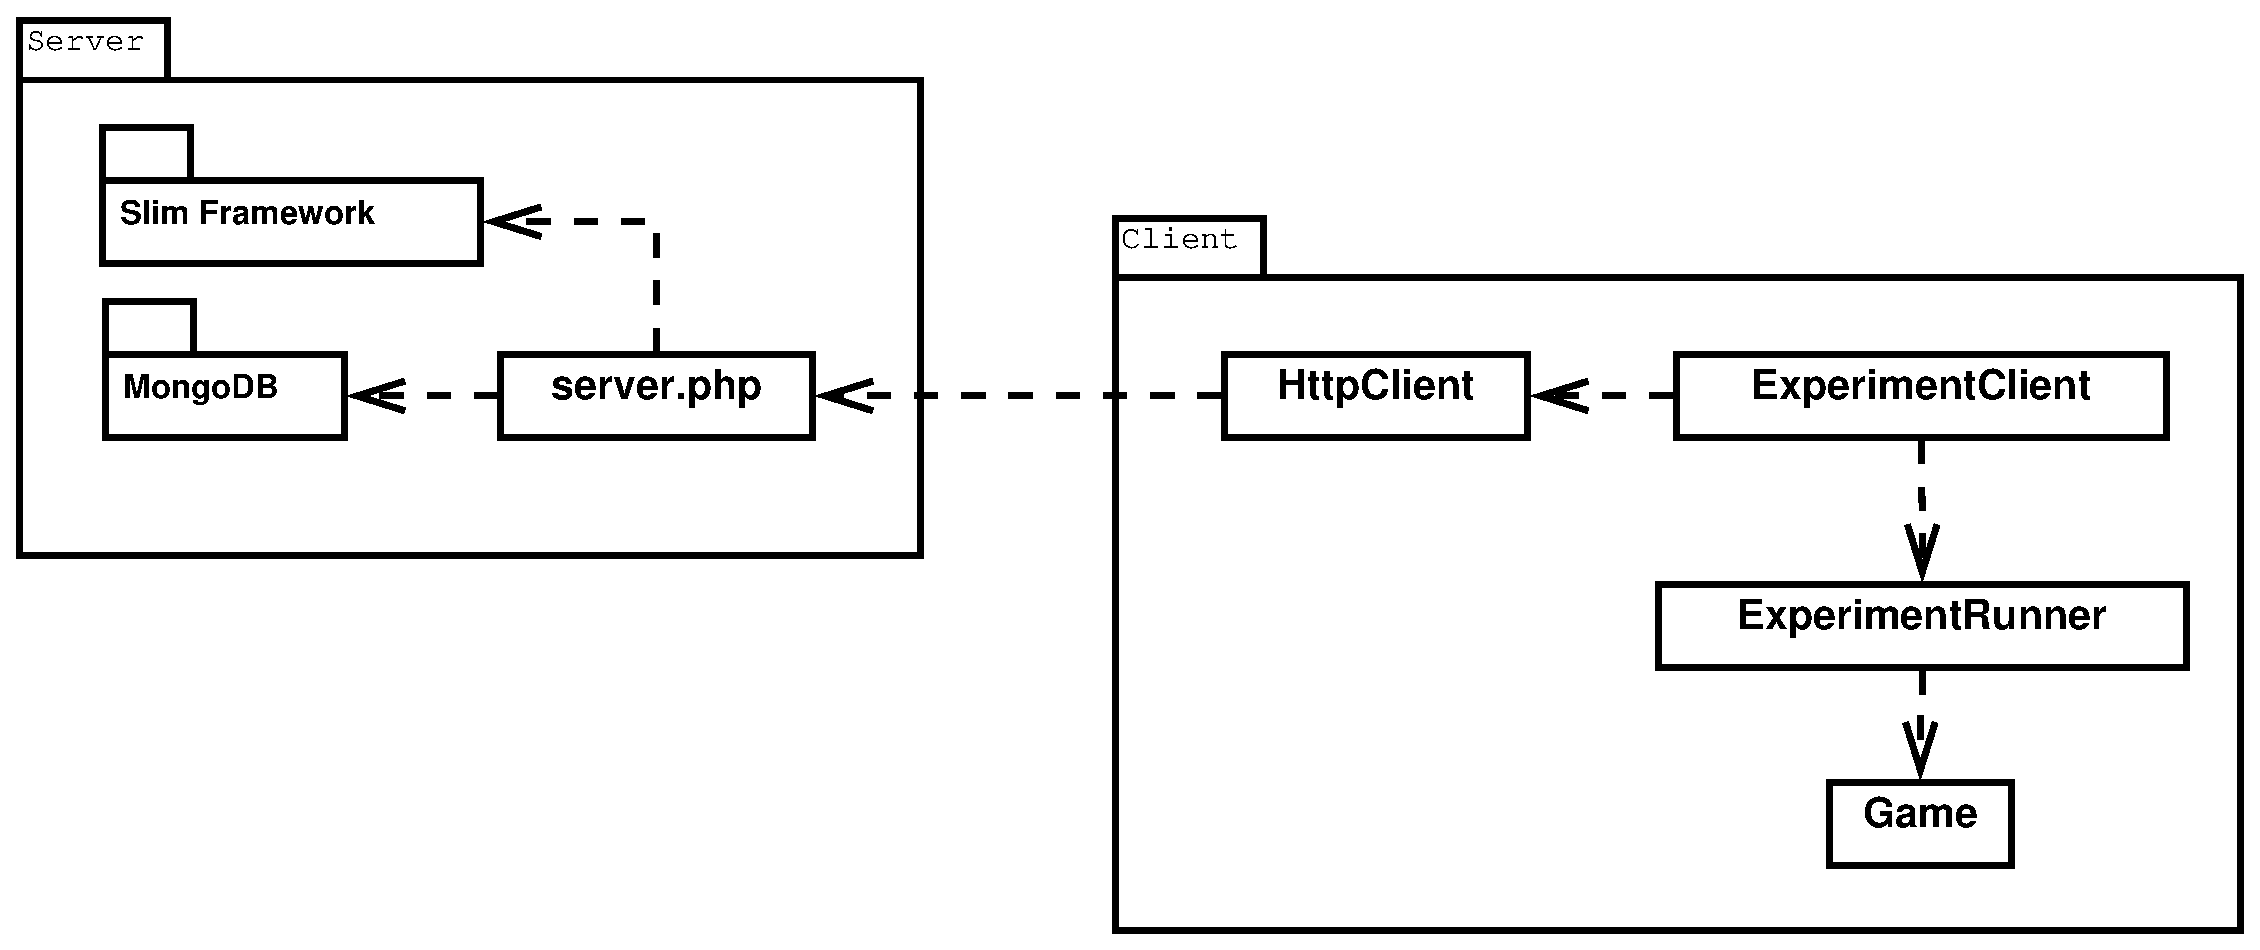
\includegraphics[width=\linewidth]{diagrams/testserver}
\caption{Test server structure}
\label{fig:testserver}
\end{figure}


The first two requirements suggest a client-server architecture, the structure of which is shown in Figure \ref{fig:testserver}.  A system was designed where experiments are stored in a MongoDB\footnote{Available at \url{http://www.mongodb.org/about/introduction/}} database with a PHP\footnote{A popular open source scripting language used mainly for web development, at \url{http://uk.php.net/}} front end, which is accessed by a Java client class.  The client class connects to the server and asks for the next available experiment: as well as an ID for the experiment, it is provided with a JavaScript snippet specifying the parameters.  More specifically, the script is run in a scope where the fields of an instance of the Parameters class, and the Java packages containing the various classes that may need to be instantiated for the parameters, are available.  Running arbitrary JavaScript may be considered overkill, however due to the time constraints on the project, it was considered a superior solution to the alternative of defining some kind of serialisation language (either on top of XML or using custom mark-up) to specify the parameters.  A typical script is shown in Listing \ref{lst:typicalscript}---note how various objects are initialised with values fed into the constructors: this would require reasonably sophisticated markup language to achieve otherwise.  The experiment object is shown in Figure \ref{fig:experiments}.

\begin{lstlisting}[breaklines=true,caption={A typical parameters script},captionpos=b,label=lst:typicalscript,float]
nodeExpansionThreshold = 30;
maximumSimulationLength = 100000;
pacManModel = new RandomNonRevPacMan();
ghostModel = new NeuralNetworkGhostController(new RouletteMoveSelectionStrategy(), 5, false);
tasks = [ ghostModel ];
selectionPolicy = new LevineUcbSelectionPolicy(4000);
opponent = new Legacy();
\end{lstlisting}

\begin{figure}
\centering
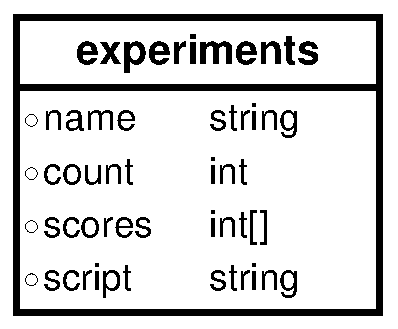
\includegraphics[scale=0.8]{diagrams/experiments}
\caption[The experiment object]{The experiment object.  The {\tt count} field starts off at the number of games that should be played with the parameters, and is decremented each time a client is given the experiment to run.  The {\tt scores} field holds the final scores for each of the games run.}
\label{fig:experiments}
\end{figure}

Several other choices were made to facilitate a quick implementation.  The chosen database system, MongoDB, is a NoSQL\footnote{NoSQL databases systems attempt to address some of the problems with traditional relational database systems (RDBMSs).  They are generally document-oriented, meaning arbitrary object graphs can be stored instead of highly structured data.  Interested readers can consult \url{http://en.wikipedia.org/wiki/NoSQL} for an overview.}, document-oriented database system which allows arbitrary denormalised object graphs to be stored.  Assuming the database server has already been installed, setup time is ostensibly nil: the program or programmer (by use of an interactive JavaScript console provided with the system) may simply start adding objects to a specified collection\footnote{A \emph{collection} is the rough equivalent of tables in a relational database system.  However, unlike tables, they do not have a precise schema, and two objects stored in the same collection may be completely different.} and a specified database name---if either of these do not exist, they are created.  By contrast, if using a system like MySQL, the programmer would have to set up the database with associated users and privileges, and execute lines upon lines of data definition language (DDL) code to create the tables.

Note also that a separate table would have to be created for the {\tt scores} field, as it is not possible to store an array of values in a SQL table.  There are ways around this---for example, one could store the scores as a comma-delimited list in a string ({\tt VARCHAR}) field, but this would greatly complicate the issue of performing numerical queries on the data.  However, the biggest issue is related to updating: if two clients finish at roughly the same time, they will both read the scores field to get its present value, add their own score to the end of the list, and save the new value.  Depending on the order of the operations, i.e., if both writes succeed both reads, one of the writes will be overwritten and the associated score will be lost.  The are also ways around this of course, but it starts to get complex here.  In contrast, MongoDB allows fields to contain arrays, and defines an atomic {\tt\$push} operator which adds a given element to an array, whilst avoiding concurrency issues.

The system makes use of MongoDB's {\tt findAndModify} operation, which updates the first document it finds matching the specified criteria and returns it, atomically.  This is useful when retrieving ``active'' experiments, that is, experiments for which the {\tt count} field has not yet been decremented to zero.  Since the sequence of actions ``search for experiment with count greater than zero'', ``decrement count'' and ``return experiment'' is executed atomically, concurrency is not an issue, and no two machines will think they are running the same experiment number.  This is also possible in SQL, but is arguably more complex.

PHP was chosen as the server-side language as it is quick to write simple websites in, and it was deemed that the rigour of a typed language was not necessary for this project.  It also allowed the Slim Framework\footnote{\url{www.slimframework.com}} to be used: this micro framework for PHP facilitates mapping URL routes for specific HTTP methods to anonymous handler functions.  This choice of framework enabled the entire application to be implemented in four short functions in a single file.  This is included as appendix \ref{ap:server}; it is easy to read and understand in its entirety, and demonstrates that the system is indeed quick to implement.

\section{Protocol details}

Three routes are handled by the application, inspired by a REST style approach:

\begin{itemize}
\item {\tt GET /active\_experiment}: find an experiment with a count greater than zero, decrement that count, and return the experiment serialised as JSON\footnote{JSON (JavaScript Object Notation) is a data interchange language which is a subset of JavaScript.  It allows objects to be serialised in the form they would take if written as a JavaScript literal, thus for example, an array of integers is simply: {\tt [1, 2, 3, 4]}.  See \url{http://www.json.org} for more details.}.  If there are no such experiments, the {\tt HTTP 410 Gone} status code is returned instead.
\item {\tt POST /experiments/\$id}: saves a score to the experiment object with the specified ID.  The body of the request should contain the score to add, serialised as JSON.
\item {\tt POST /experiments}: saves an experiment to the collection of experiments.  The experiment to save should be included in the body of the request, serialised as JSON.
\item {\tt GET /experiments}: gets the full list of experiments including scores.
\end{itemize}

The Java client retrieves an experiment using the first route, runs the game, and when it has completed, saves the final score using the second route.  The third route was added for convenience to allow a small utility programme on the client to upload experiment scripts specified in files, and the fourth to allow the scores data to be retrieved easily.

\section{Summary}

This chapter has described the implementation of an ``experiment server'' which distributes games over many computers.  Around 2000 games were palyerd to evaluate the project, and this was completed over a couple of days rather than the 1--2 weeks it would take on one machine.  Considering that it took only an adfternoon to implement, the experiment server is considered a particular success.  The results gathered using this server are presented and discussed in the next chapter.



